\documentclass[aps,prd,twocolumn,superscriptaddress,amsfont,amssymb,amsmath,nofootinbib,showpacs,balancelastpage]{revtex4-1}
%\documentclass[prd,superscriptaddress,twocolumn,floatfix]{revtex4}

\usepackage{graphicx,longtable,natbib,mathrsfs,color}
\usepackage{txfonts}

\newcommand{\bs}{\boldsymbol}
\newcommand{\diff}{{\mathrm d}}
\newcommand{\Cov}{\mathsf{C}}
\newcommand{\Fish}{\mathsf{F}}
\newcommand{\Cl}{\mathcal {C}}
\newcommand{\R}{\mathcal{R}}
\newcommand{\T}{\mathcal{T}}
\newcommand{\Msun}{M_\odot}

%
\def\apjl{Astrophys. J. Lett.}
\def\apjs{Astrophys. J. Suppl. Ser.}
\def\aj{Astron. J.}
\def\mnras{Mon. Not. R. Astron. Soc.}
\def\aap{Astron. Astrophys.}                % Astronomy and Astrophysics
\def\jcap{J. Cosmology Astropart. Phys.}
\def\aapr{Astron. Astrophys. Rev.}

\begin{document}

\addtolength{\hoffset}{-0.525cm}
\addtolength{\textwidth}{1.05cm}
\title{Displacement field paper}

%\author{Hao-Ran~Yu} \affiliation{}\email{haoran@cita.utoronto.ca}
%\author{Qiaoyin~Pan}
%\author{Ue-Li~Pen} \affiliation{}
%\author{Tong-Jie~Zhang} \affiliation{}
%---


%\date{Received \today; published -- 00, 0000}

\begin{abstract}
Abstract goes here.
\end{abstract}

%\pacs{98.80.Es 95.36.+x}

\maketitle

\section{Introduction}\label{sec.intro}
Introduction goes here. Citation \cite{2000ApJ...534L..19P}. Bold type use $\bs{v}=\vec{v}$.

\section{Method}\label{sec.method}
Method goes here.


\begin{figure} \centering
  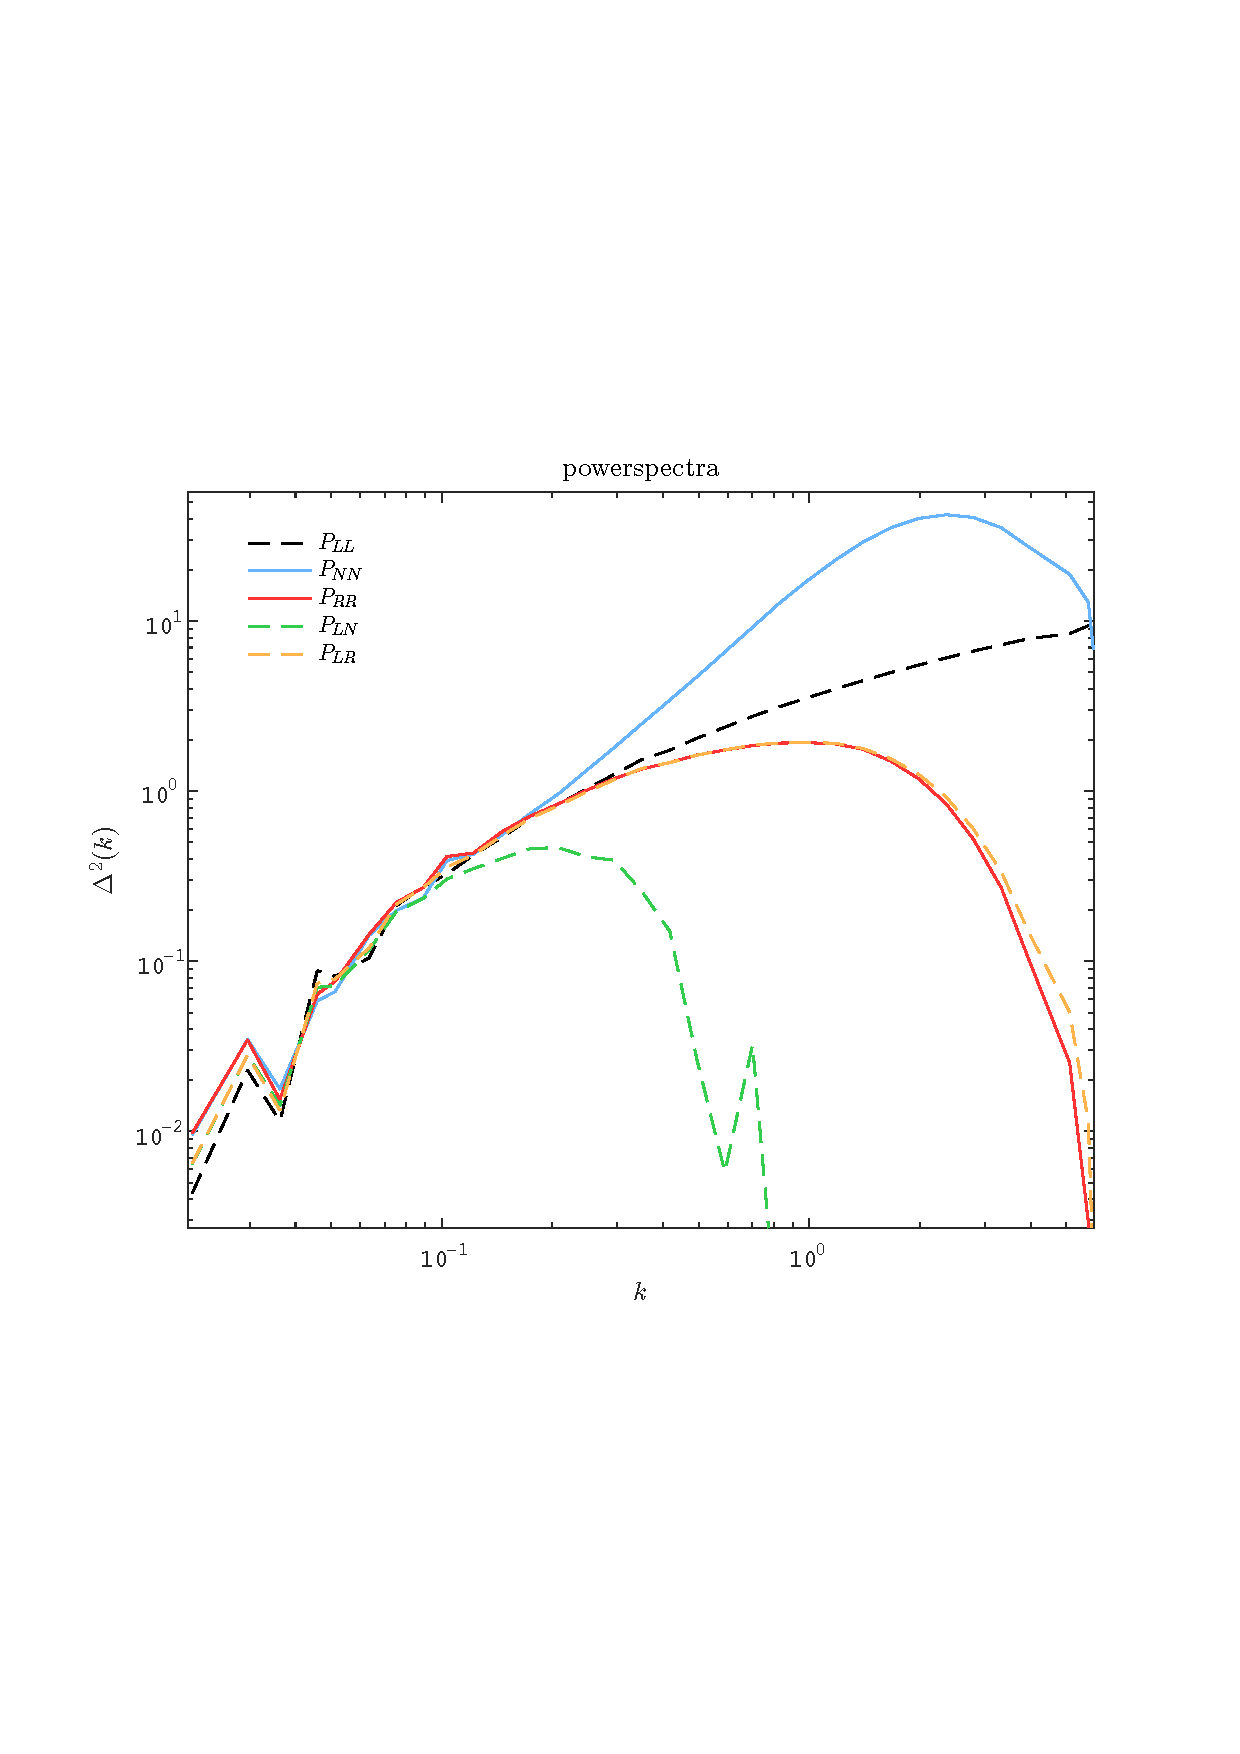
\includegraphics[width=1.0\linewidth]{fig1.pdf}
  \caption{Caption goes here.}
  \label{fig.1}
\end{figure}


\section{Discussion and conclusion}\label{sec.discussion}
Discussion goes here.

\section*{Acknowledgements}
Acknowledgements goes here.

%\bibliographystyle{apsrev4-1}
\bibliographystyle{h-physrev3}
\bibliography{../haoran_ref}

\end{document}
